\documentclass[12pt]{beamer}

% \usepackage[margin=1in]{geometry}
\usepackage{parskip}
\usepackage{amssymb}
\usepackage{mathtools}
\usepackage{matlab-prettifier}
\usepackage{multimedia}

\author{Matt Cho}
\title{Simulating a Droplet Within a Two-phase Viscous Flow}
\date{}
\usetheme{Rochester}
\usecolortheme{lily}
\setbeamertemplate{navigation symbols}{}

\begin{document}
\maketitle

% Analytical Method vs Exploratory Analysis
% Modern Analysis vs "Post-Moore's Law"-Analysis
\begin{frame}
    \frametitle{CFD Methodology}

    We have a mental model. Is it closer to what we think is real or not?
\end{frame}
\begin{frame}
    \frametitle{CFD Methodology}
    \underline{Scientific Method}

    Analytical method where we go through an iterative process of:

    \textbf{Question $\rightarrow$ Hypothesis $\rightarrow$ Experiment $\rightarrow$ Refinement}

    (Engineering methodology is identical, but with cost constraints added.)
\end{frame}
\begin{frame}
    \frametitle{CFD Methodology}
    \underline{Scientific Method}

    
\includegraphics[width=0.7\textwidth]{img/0-caltech-maxwell.png}
\end{frame}
\begin{frame}
    \frametitle{CFD Methodology}
    \underline{Computational Math ("Post-Moore's Law")}

    We have a virtual model written in the form of an algorithm. How do we make the most of it?
\end{frame}
\begin{frame}
    \frametitle{CFD Methodology}
    \underline{Computational Math ("Post-Moore's Law")}

    Process is fundamentally the same, but we now have 1000s of CPUs to do 
    what we want:

    \textbf{Question $\rightarrow$ Hypothesis $\rightarrow$ Experiment $\rightarrow$ Experiment $\rightarrow$ Experiment $\rightarrow$ Experiment $\rightarrow$ Experiment $\rightarrow$ \dots}
\end{frame}
\begin{frame}
    \frametitle{CFD Methodology}
    \underline{Computational Math ("Post-Moore's Law")}

    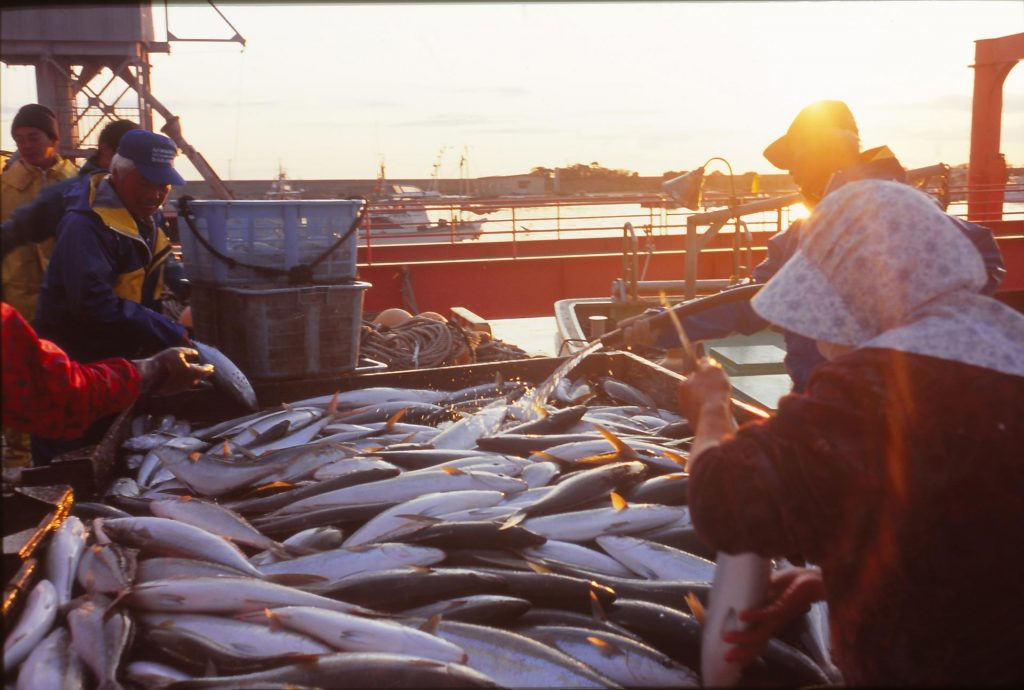
\includegraphics[width=0.7\textwidth]{img/1-fisher.jpg}
\end{frame}
\begin{frame}
    \frametitle{CFD Methodology}
    \underline{Computational Math ("Post-Moore's Law")}

    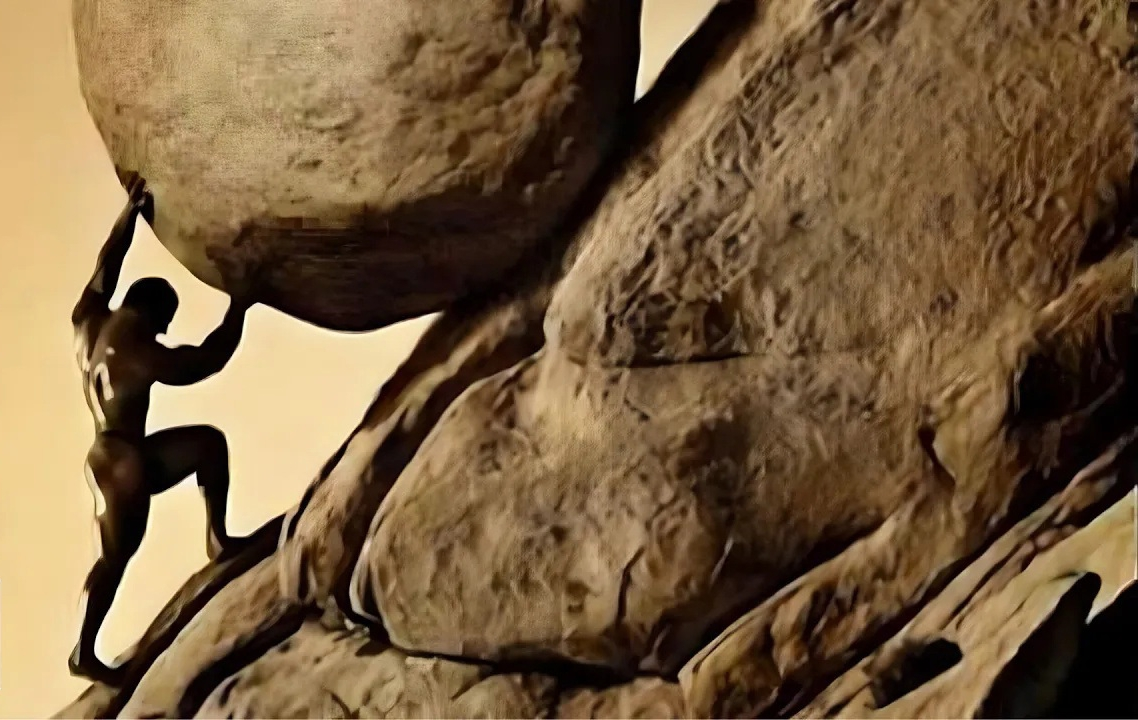
\includegraphics[width=0.7\textwidth]{img/2-sisyphus.jpg}
\end{frame}

% Introducing software framework, Basilisk
\begin{frame}
    \frametitle{Software Framework}
    \underline{Introducing Basilisk}

    General Purpose PDE Solver specializing in solving over adaptive meshes.

    Creator is Stéphane Popinet of Sorbonne Université (formerly Université Pierre-et-Marie-Curie) in Paris
\end{frame}
\begin{frame}
    \frametitle{Software Framework}
    \underline{Introducing Basilisk}

    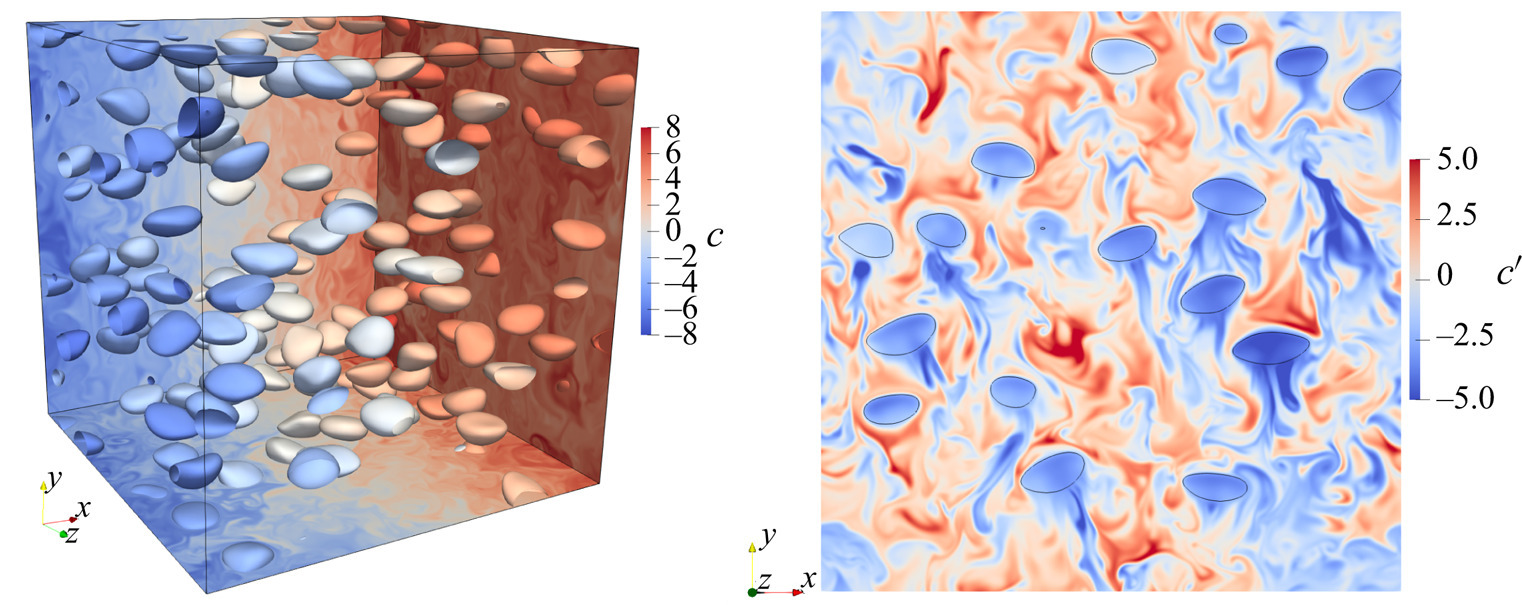
\includegraphics[width=\textwidth]{img/3-hidman2023.jpg}
\end{frame}
\begin{frame}
    \frametitle{Software Framework}
    \underline{Introducing Basilisk}

    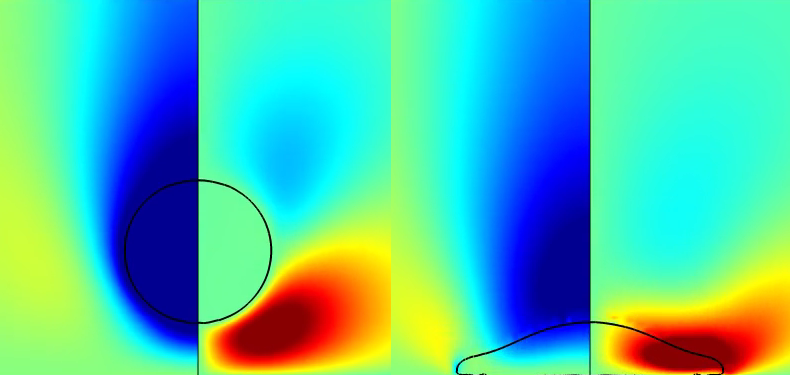
\includegraphics[width=\textwidth]{img/4-drop.png}
\end{frame}
\begin{frame}
    \frametitle{Software Framework}
    \underline{What is this really?}

    A solution to the Navier-Stokes equations,
    using the Volume-of-Fluid method (VOF).
\end{frame}
\begin{frame}
    \frametitle{Software Framework}
    \underline{What is this really?}

    A solution to the Navier-Stokes equations,
    using the Volume-of-Fluid method (VOF).

    Problem of analysing real droplet behavior is a combination of problems. In 
    isotropic conditions, this is essentially solving for a two-phase flow 
    problem where the substrate is a solid boundary.

    (We are interested in viscosity and advection more than heat transfer.)
\end{frame}
\begin{frame}
    \frametitle{Software Framework}
    \underline{What is this really?}

    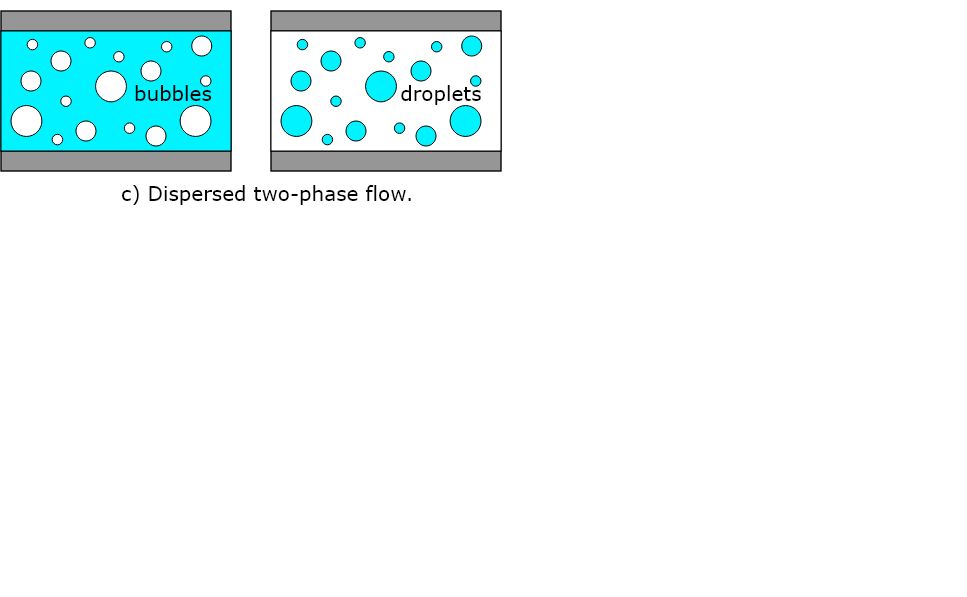
\includegraphics[width=1.75\textwidth]{img/6-twophase.png}
\end{frame}

\begin{frame}
    \frametitle{Current Work: 2-D Simulation}
    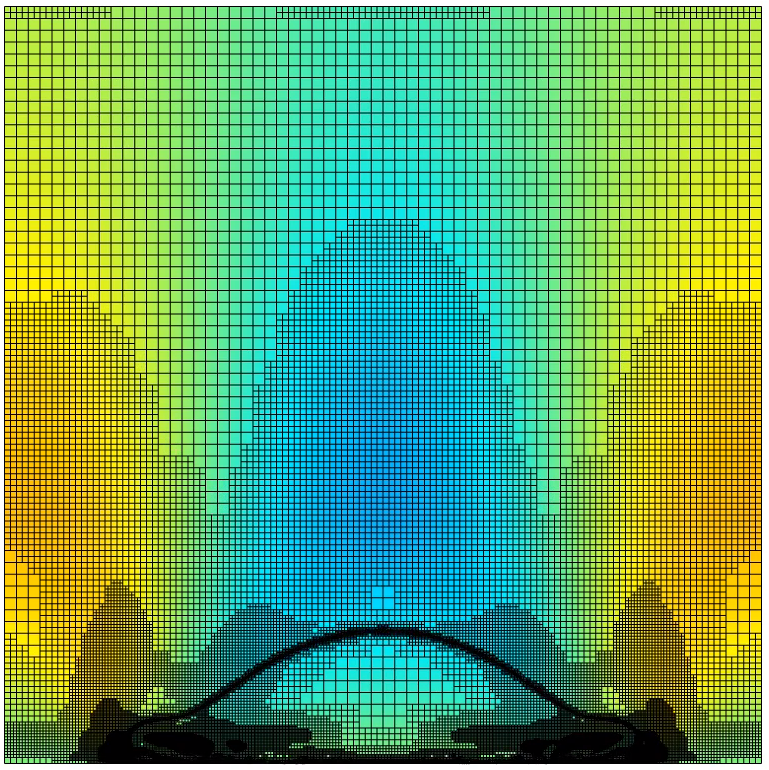
\includegraphics[width=0.7\textwidth]{img/7-current.png}
\end{frame}
\begin{frame}
    \frametitle{Current Work: 2-D Simulation}
    \underline{Some Problems and Solutions:}

    - Even for symmetric problems, mirroring a simpler domain isn't sufficient.
\end{frame}
\begin{frame}
    \frametitle{Current Work: 2-D Simulation}
    \underline{Some Problems and Solutions:}

    - Even for symmetric problems, mirroring a simpler domain isn't sufficient.

    - At small length scales, numerical errors dominate the physics unless if 
    they are mitigated.
\end{frame}
\begin{frame}
    \frametitle{Current Work: 2-D Simulation}
    \underline{Some Problems and Solutions:}

    - Even for symmetric problems, mirroring a simpler domain isn't sufficient.

    - At small length scales, numerical errors dominate the physics unless if 
    they are mitigated.
    
    - Experiment Design: Trying to match real conditions is incredibly 
    computationally intensive, have to settle for simpler model with respective 
    changes in non-dimensional numbers.
\end{frame}

\begin{frame}
    \frametitle{Results and Future Work}
    Currently have a fairly reasonable simulation of a "nanodroplet" (micro and
    nanometer length scale) that agrees with constants reported in literature.
\end{frame}
\begin{frame}
    \frametitle{Results and Future Work}
    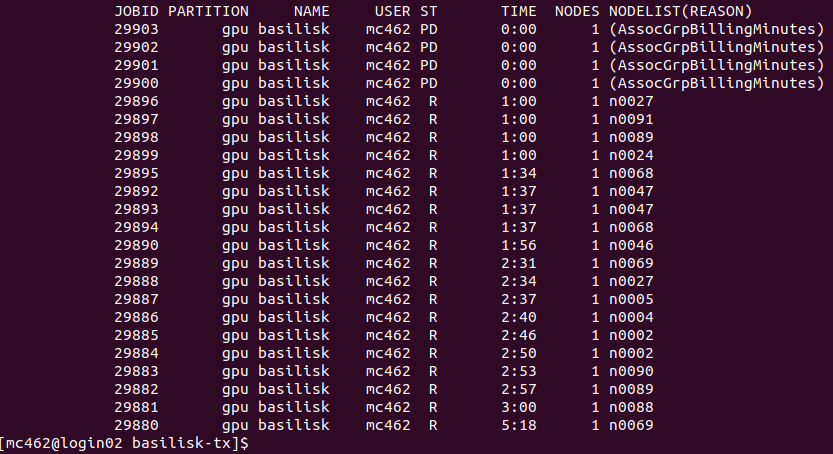
\includegraphics[width=0.75\textwidth]{img/8-slurm.png}
\end{frame}
\begin{frame}
    \frametitle{Results and Future Work}
    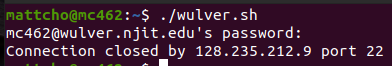
\includegraphics[width=0.9\textwidth]{img/9-njit.png}
\end{frame}
\begin{frame}
    \frametitle{Results and Future Work}
    Currently have a fairly reasonable simulation of a "nanodroplet" (micro and
    nanometer length scale) that agrees with constants reported in literature.

    Natural thing to do would be to incrementally approach larger scale 
    (mm length).
\end{frame}
\begin{frame}
    \frametitle{Results and Future Work}
    Currently have a fairly reasonable simulation of a "nanodroplet" (micro and
    nanometer length scale) that agrees with constants reported in literature.

    Natural thing to do would be to incrementally approach larger scale 
    (mm length).

    The way forward is then to apply tried and true computer 
    programming/engineering techniques to make computational problem tractable.
\end{frame}


\end{document}
    